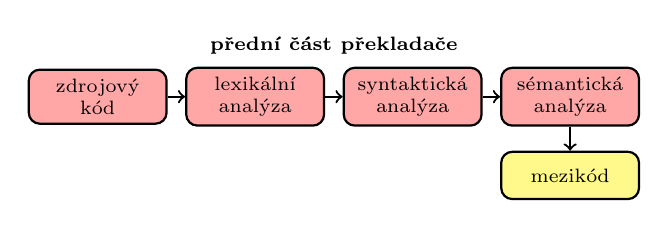
\begin{tikzpicture}[
    box/.style={
        draw,
        rounded corners,
        thick,
        align=center,
        font=\scriptsize,
        minimum width=1.75cm,
        minimum height=0.6cm
    },
    arrow/.style={->, thick}
]

    \node<2->[box, fill=red!35] (src) at (0,0) {zdrojový\\kód};
    \node<2->[box, fill=red!35] (lex) at (2.0,0) {lexikální\\analýza};
    \node<2->[box, fill=red!35] (syn) at (4.0,0) {syntaktická\\analýza};
    \node<2->[box, fill=red!35] (sem) at (6.0,0) {sémantická\\analýza};
    \node<3->[box, fill=yellow!45] (ir) at (6.0,-1.0) {mezikód};

    \draw<2->[arrow] (src) -- (lex);
    \draw<2->[arrow] (lex) -- (syn);
    \draw<2->[arrow] (syn) -- (sem);
    \draw<3->[arrow] (sem) -- (ir);

    \node<2->[font=\scriptsize\bfseries] at (3.0,0.65) {přední část překladače};

\end{tikzpicture}
